
\documentclass[12pt]{article}
\usepackage{siunitx} 
\usepackage{graphicx} 
\usepackage{amsmath} 
\setlength\parindent{24pt} 
\usepackage[top=0.5in,bottom=2in,left=1.25in,right=1.25in, includehead,includefoot,a4paper]{geometry}
\usepackage{times} 


\title{Determination of the Refractive Indexes \\ of Air and Acrylic \\ }
\author{Yi \textsc{Hu}} 
\date{\today} 



\begin{titlepage}
\begin{document}
		\maketitle 
		\thispagestyle{empty}

	
	\begin{center}
		\begin{tabular}{l r}
			Date Performed: & March 2, 2016 \\ % Date the experiment was performed
			Partners: & Yi Hu \\ % Partner names
			& Trina Le \\
			Instructor: & Kyle Slinker % Instructor/supervisor
		\end{tabular}
	\end{center}
\end{titlepage}




%----------------------------------------------------------------------------------------
%	SECTION 1
%----------------------------------------------------------------------------------------
\section{Abstract}
We determined the index of refraction of air and an acrylic sheet with a Michelson interferometer. For air, the relation between the change in air pressure within a chamber and the number of fringes (of the interference image) was used for calculation. We determined the refractive index of air to be $1.0003\pm0.0104$ and the major source of uncertainty the random uncertainties of instrument resolution and miscounting. For acrylic, the incident angle and the corresponding number of fringes were used to determine the refractive index. Our result was $1.43\pm0.04$, which failed to include the expected value. We concluded our major uncertainty to be systematic from our theoretical model of linear function.  

%----------------------------------------------------------------------------------------
%	SECTION 2
%----------------------------------------------------------------------------------------
\section{Theory}
The index of refraction $n$ is the ratio of the speed of light in a vacuum $c$ to the speed of light in a medium $v$. $n=\dfrac{c}{v}$. When light passes through a different medium, it will bend as the wavelength $\lambda$ changes. In this experiment, we used this property of light to measure the refractive indexes of air and acrylic sheet with a Michelson Interferometer for the observation of the interference pattern.

%----------------------------------------------------------------------------------------
%	SECTION 2.1
%----------------------------------------------------------------------------------------
\subsection{Michelson Interferometer}
The Michelson Interferometer is shown next page in Fig.1. When the source light passed through the splitter, half headed toward mirror 1 while the other half was reflected toward mirror 2. When these two beams reflected back by the mirrors, they met and were superimposed, creating a fringe pattern of interference. In the bright regions of the pattern, the crests of the waves of the two beams arrive together. In the dark areas, the crest of one wave arrives at the same time as the trough of the other. 

In this lab, we did not change the physical path length of the beams, but instead changed the optical path length $\tau$. The optical path length of light passing through multiple mediums is equal to $\Sigma n_{i}L_{i}$, where $n_{i}$ is the refractive index of the each individual medium and $L_{i}$ is the physical path length within the medium. If the optical path length of one beam changes by one wavelength, the interference pattern is shifted by one fringe. 
\begin{figure}[htb]
	\begin{center}
		\includegraphics[width=0.40\textwidth]{picture1} % Include the image placeholder.png
		\caption{Michelson Interferometer.}
	\end{center}
\end{figure}

%----------------------------------------------------------------------------------------
%	SECTION 2.2
%----------------------------------------------------------------------------------------
\subsection{Index of Refraction of Air}
To determine the index of refraction of air, we altered the optical path length by placing a vacuum chamber in front of one of the mirrors, as shown in Fig. 2, and pumped out the air slowly. In this way, we changed the optical path length of one beam by creating a vacuum environment halfway through, but left that of the other beam unchanged. This resulted in a shift in the observed interference pattern of constructive and destructive interference. 

\begin{figure}[htb]

	\begin{center}
		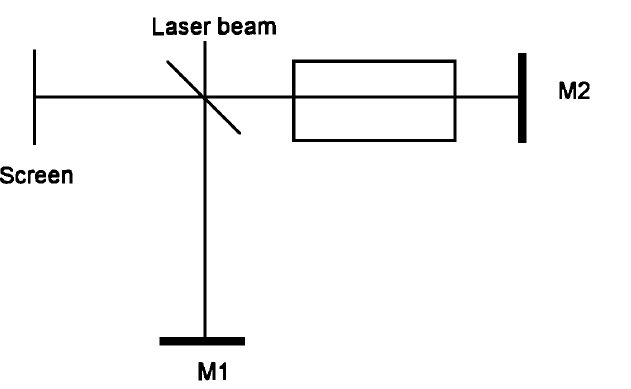
\includegraphics[width=0.65\textwidth]{picture2} % Include the image placeholder.png
		\caption{The setup for determining the refractive index of air.}
	\end{center}
\end{figure}

For air and other ideal gases, the difference between the refractive index and 1 (which is the refractive index of vacuum) is proportional to the pressure of the gas. Thus the index of refraction within the chamber dropped slowly as the pressure decreased, and reached 1 when all the air was pumped out. Suppose the refraction index of air is $n$, and the air pressure is $p$, then we have
\begin{equation}
	n=1+cp
\end{equation}

where $c$ is an unknown constant. 

So when the pressure is changed, the corresponding change in the refraction index is
\begin{equation}
\Delta{n}=c\Delta{p}
\end{equation} 

In our experiment, the optical path length within the chamber is $nL$, where $n$ is the refractive index and $L$ is the length of the chamber. Since the beam passed through the chamber twice, and the refractive index changed from that of the air to that of vacuum, we altered the optical path length by $2L\Delta{n}$, in which $\Delta{n}$ is the change in refractive index caused by the change in pressure. 
\begin{equation}
	\Delta{\tau}=2L\Delta{n}
\end{equation}

On the other hand, as the air was being removed, the interference pattern would shift by one fringe at each time the optical path length was changed by one wavelength $\lambda$. So the relation between the observed number of shifts in fringes $m$ and the change in optical path length is 
\begin{equation}
	\Delta{\tau}=m\lambda
\end{equation}

Based on Equ.(2),(3), and(4), we get the unknown constant $c$ to be 
\begin{equation}
	c=\dfrac{m\lambda}{2L\Delta{p}}
\end{equation} 
and if we measured $m$ fringes while the pressure changed by an amount of $\Delta{p}$, by plotting $m$ as a function of $\Delta{p}$, we have 
\begin{equation}
	m=\dfrac{2Lc}{\lambda}\Delta{p}
\end{equation}
with the slope $k=\dfrac{2Lc}{\lambda}$. Expressing $c$ in terms of the slope $k$ gives $c=\dfrac{k\lambda}{2L}$. Thus we can calculate the index of refraction for air at room temperature to be 
\begin{equation}
	n_{air}=\dfrac{k\lambda{p}}{2L}+1
\end{equation}
in which $p$ is the atmosphere pressure.

%----------------------------------------------------------------------------------------
%	SECTION 2.3
%----------------------------------------------------------------------------------------
\subsection{Index of Refraction of Acrylic}
To measure the refractive index for acrylic, we replaced the vacuum chamber by a rotation stage that held an acrylic sheet and measured the angle through which it had been turned. Under this setup, we changed the optical path length of one beam by rotating the acrylic sheet. For the same reason that we only changed the path length of one beam, a shift in the interference pattern could be observed and recorded for the calculation of of the refractive index of acrylic. 

Suppose the thickness of the acrylic sheet is $t$ and OP is the original direction of light normal to the sheet, as shown in Fig. 3. Since the refractive index of the air is very close to that of vacuum, we can reasonably assume the index of refraction of air to be 1. Thus the total optical path length between a and c initially for the propagation of light is $nt+bc$ in which $n$ is the index of refraction of acrylic. When acrylic sheet is rotated through an angle $i$, the angles of incidence and refraction are $i$ and $r$ respectively (when the light beam first encounters the acrylic sheet), and the optical path length becomes $ad*n+de$.

\begin{figure}[htb]
	\begin{center}
		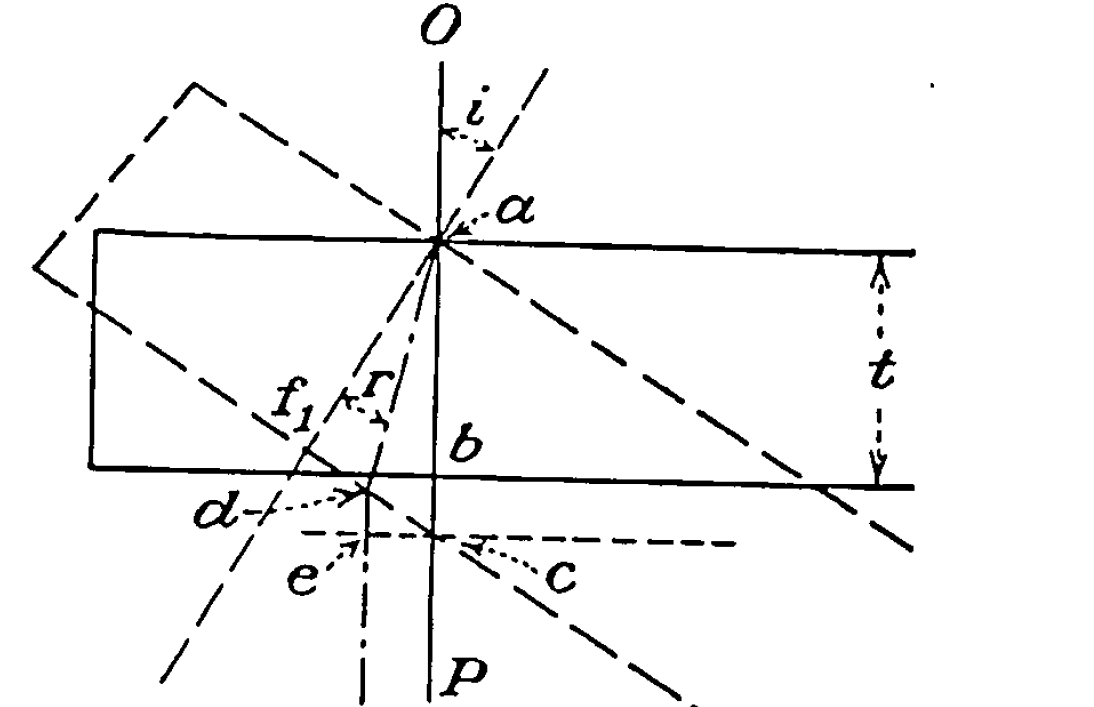
\includegraphics[width=0.5\textwidth]{picture4} % Include the image placeholder.png
		\caption{A light beam travels through an acrylic sheet.}
	\end{center}
\end{figure}

So the change in optical path length equals
\begin{equation}
	\Delta{\tau}=2(n\times{t}+bc-ad\times{n}-de)
\end{equation}
the path length is doubled because the light beam goes through the sheet twice.

Based on the trangles in Fig. 3, we have $ ad=\dfrac{t}{\cos{r}} $, $ bc= \dfrac{t}{\cos{i}}-t$, and $ de=cd\sin{i}=(cf-df)\sin{i}$, in which $cf=t\tan{i}$ and $df=t\tan{r}$. With these relations we get
\begin{equation}
	\Delta{\tau}=2(n{t}+\dfrac{t}{\cos{i}}-t-\dfrac{nt}{\cos{r}}-t\dfrac{sin{i}^{2}}{\cos{i}}+t\tan{r}\sin{i})
\end{equation}



Snell's Law gives
\begin{equation}
	\sin{i}=n\sin{r}
\end{equation}

Combine Equ.(8) and the relation between the observed number of shifts in fringes $m$ and the change in optical path length $\Delta{\tau}=m\lambda$ we get
\begin{equation}
\dfrac{m\lambda}{2t}=n-1+\sec{i}-\tan{i}\sin{i}+\tan{r}\sin{i}
\end{equation}
with Snell's law and the relation $\sin{r}^{2}+\cos{r}^{2}=1$ we substitute all the $r$ with $i$ and get the relation 
\begin{equation}
\dfrac{m\lambda}{2t}=n+\cos{i}-1-\sqrt{n^{2}-\sin{i}^{2}}
\end{equation}

Solving the equation gives us the relation between the refractive index $n$ and the number of fringes
\begin{equation}
	n=\dfrac{(2t+m\lambda)(1-\cos{i})+(\dfrac{m\lambda}{2t})^{2}}{2t(1-\cos{i})+m\lambda}
\end{equation}

Since $\dfrac{m\lambda}{2t}$ is a small number and its square is close to zero, we approximate $n$ to be 
\begin{equation}
n=\dfrac{(2t+m\lambda)(1-\cos{i})}{2t(1-\cos{i})+m\lambda}
\end{equation}

If we keep the angle of incidence small, we can use a Taylor expansion to approximate $\cos{i}$ to be $1-\dfrac{i^{2}}{2}$, thus we have
\begin{equation}
	m\lambda=2ti^{2}\dfrac{n-1}{2n+i^{2}}
\end{equation}
and $i^{2}$ in the denominator is relatively small compared to $2n$ for small angle, so we can further approximate the relation between the number of fringes and the square of incidence angle to be
\begin{equation}
	m=\dfrac{t(n-1)}{\lambda{n}}i^{2}
\end{equation} 

Fnally, if we plot $m$ as a function of $i^{2}$, the slope $k$ will be
\begin{equation}
	k=\dfrac{t(n-1)}{n\lambda},
\end{equation}
which means the index of refraction of acrylic $n$ to be 
\begin{equation}
	n=\dfrac{t}{t-k\lambda}.
\end{equation}

%----------------------------------------------------------------------------------------
%	SECTION 3
%----------------------------------------------------------------------------------------
\section{Procedure}
In this lab, we used a Michelson interferometer, a HeNe laser, a vacuum chamber and a acrylic sheet to measure the refractive index of air and acrylic. 
\begin{enumerate}
	\begin{item}
	 to measure the index of refraction of air
	\end{item}
	\begin{item}
		to measure the index of refraction of an acrylic sheet
	\end{item}
\end{enumerate}

For the determination of refraction index of air, we shined the laser at the Michelson interferometer with a vacuum chamber put in the path of one of the interferometer arms, as shown in Fig. 2. For the acrylic, we replaced the vacuum chamber with a acrylic sheet mounted on a rotation stage. 
\subsection{Alignment}
To create an interference pattern, the interferometer must be aligned before both experiment \textit{\textbf{a}} and \textit{\textbf{b}}. We first set up the equipment as shown in Fig. 2. Then we plugged in and turned on the laser. Attention should be paid to not looking directly into the laser beam. 

Since we could not look in the interferometer directly when using a laser, we placed a box as a screen and shined the result pattern onto it. A small lens was used to spread the laser beam passing through the interferometer. 

We covered mirror 1 with a sheet of paper. In this way, only the laser beam that headed toward mirror 2 was reflected. We adjusted the location and orientation of the laser until the return beam was very close to the exit hole on the face of the laser. Some light from mirror 2 could be observed on the screen. 

Then we uncovered the mirror 1. This led to another set of light seen on the screen. We turned the screws on mirror 1 until the two sets of light superimposed and an interference pattern of concentric fringes was shown on the screen after we had aligned the interferometer properly. 

\subsection{Experiment a: measure the refraction index of air }
With a vacuum chamber set in the path of one of the interferometer arms, we first aligned the interferometer. Then we opened the chamber several times to make sure the pressure inside and outside the chamber were the same at the beginning of our experiment.

Then, while observing the interference pattern projected on the box, we squeezed the handle of the vacuum pump to pump out the air inside the chamber. We stopped evacuating the chamber for every  5 passing fringes and recorded the reading of the vacuum gauge which showed the difference between the pressure within the chamber and the pressure outside.

The greater the difference in pressure, the slower the chamber was being evacuated (because of the force caused by the pressure) and the slower the fringes passed by. So when the pressure inside the chamber dropped to $40\%$ of the outside air pressure, we recorded the reading on the vacuum gauge for every 2 fringes.  

Finally we plotted the number of fringes as a function of difference in pressure and calculated the refractive index of air based on Equ. (7). 

\subsection{Experiment b: measure the refraction index of an acrylic sheet }
After experiment \textbf{a}, we replaced the vacuum chamber with a rotation stage on which we placed a sheet of acrylic and re-aligned the Michelson interferometer. 

To make the sheet normal to the incoming ray at first, we slowly rotated the rotation stage until a point where changing the direction of the rotation did not change the moving direction of the fringes (i.e. a position of the shortest path length where slightly changing the orientation in either direction resulted in an increase in path length). Then we recorded this position as the initial situation based on the reading on the rotation stage. 

Then we began rotating the sheet manually towards one side so that the fringes started collapsing or appearing on the screen. The number of passing fringes, for every $\SI{2}{\degree}$ angle the rotation stage was rotated, was noted down carefully. We only recorded data of which the angle displacement was smaller than $\SI{20}{\degree}$ because we applied small angle approximation in our theory.

Finally, by sifting out useful data points and plotting the number of passing fringes as a function of incident angle (in radian), we calculated the refractive index of acrylic based on Equ. (18).



%----------------------------------------------------------------------------------------
%	SECTION 4
%----------------------------------------------------------------------------------------
\section{Analysis}

\subsection{The index of refraction of air}

We recorded the number of passing fringes and the change in pressure as we pumped out the air within the vacuum chamber. The length of the vacuum chamber used was given $L=0.05\si{m}$ and the wavelength of HeNe laser we used was \SI{632.8}{\nano\meter}. Our data is shown below in Table 1.
\begin{table}[!hb]
		
	\begin{center}
		 \caption{The number of collapsing fringes with the corresponding change in pressure. }
			\begin{tabular}{|c|c|c|c|c|c|c|c|c|c|c|c|}
				\hline\hline
			Trials	& 1 & 2 & 3 & 4&5&6&7&8&9&10&11\\ \hline
				Number of fringes  $m (\pm{1})$&0&5&10&15&20&25&27&29&31&33&35\\ \hline
				Change in pressure $\Delta{p}(\pm{2}) [\si{\kilo\pascal}]$ &0&13&24&36&47&60&65&72&76&80&84\\
				\hline
			\end{tabular}
	\end{center}
\end{table}

We recorded the decrease (from the room atmosphere pressure) in air pressure for every certain count of fringes (beginning with every 5 counts and later 2 counts). The uncertainty for the fringes was considered to be 1 because we determined we might miscount 1 at most for every 5 counts. The uncertainty of $\Delta{p}$ was 2 \si{kPa} determined by the resolution of the equipment. 

By plotting, we got the best fit line with slope of $0.412$ and y-intercept of $0.025$, as shown in Figure 4. The uncertainties of $m$ and $\Delta{p}$ were shown as error bars. Using LINEST function in Excel, we determined the uncertainty associated with the slope to be $0.004$ and with y-intercept $0.247$. 

\begin{figure}[!hbt]
	\begin{center}
		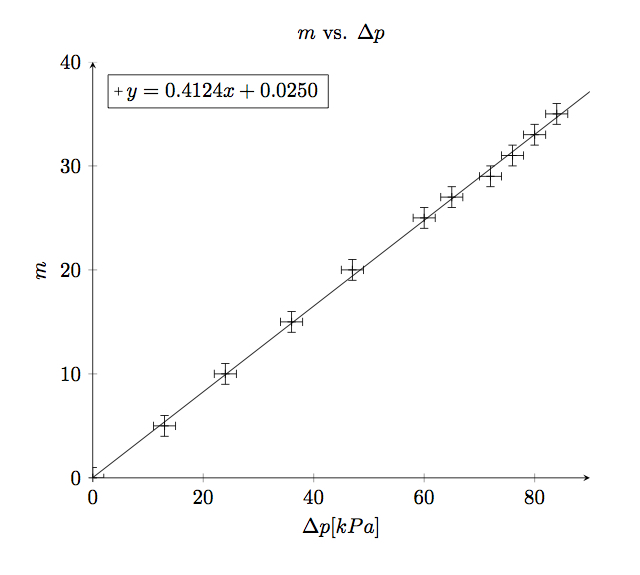
\includegraphics[width=10cm]{mp}
		\caption{The number of collapsing fringes with the corresponding change in pressure.}
	\end{center}
\end{figure}

The fact the value of y-intercept was smaller than it's uncertainty was consistent with our theory that the number of fringes is proportional to the change in pressure. 

With slope $k=0.412\pm0.025$, we calculated the refraction index of air based on equation (7) using the standard atmosphere pressure $p=101.325\si{kPa}$

\begin{equation}
n_{air}=\dfrac{k\lambda{p}}{2L}+1=1.0003.
\nonumber
\end{equation}

The uncertainty was propagated using quadrature and mainly depended on the uncertainty of $k$, which had a large relative uncertainty of $1.04\%$. 
Uncertainty calculation is shown below:
\begin{equation}
	\dfrac{\sigma_{n_{air}}}{n_{air}}=\dfrac{\sigma_{k}}{k}=1.04\%
	\nonumber
\end{equation}
\begin{equation}
		\sigma_{n_{air}}=0.0104.
		\nonumber
\end{equation}

So our result for the index of refraction of air is $1.0003\pm{0.0104}$.  The expected value is 1.00029, which lies within our uncertainty range.

\subsection{The index of refraction of an acrylic sheet}

After setting the initial orientation of the acrylic sheet to be normal to the incident light, we recorded the number of fringes collapsing or appearing for every \SI{2}{\degree} by which the rotation stage had been rotated. The angle displacements were measured in degrees, with uncertainty of $2$\si{\degree} given by the resolution of the equipment. The thickness of the acrylic sheet was measured by a micrometer with a resolution of $\SI{0.02}{mm}$ and the thickness to be  $t=1.76\pm0.02$\si{nm}. We used mercury's green emission line, with the given wavelength $\lambda=\SI{546}{nm}$. Our measured data was shown in Table 2. 

\begin{table}[!hb]
	
	\begin{center}
		\caption{The number of collapsing fringes with the corresponding angle displacement. }
		\begin{tabular}{|c|c|c|c|c|c|c|c|c|c|c|c|}
			\hline\hline
			& 1 & 2 & 3 & 4&5&6&7&8&9&10&11\\ \hline
			Angle displacement $(\pm{4}) [\si{\degree}]$ &0&2&4&6&8&10&12&14&16&18&20\\
			\hline
			Number of fringes $m (\pm{3})$&0&5&10&16&26&34&44&51&62&75&90\\ \hline
			
		\end{tabular}
	\end{center}
\end{table}

Due to the unstableness of the rotation stage, it was hard to control its rotation. So we determined the uncertainty of the angle displacement to be greater than the resolution of equipment and set to \SI{4}{\degree}. It also made counting fringes harder since we barely rotated the stage smoothly and the projected image was flashing sometimes. Thus we determined the uncertainty caused by miscounting regarding the number of fringes to be 3. 

The angle displacement of the rotation stage was equal to the incident angle $i$. We converted the units into \si{\radian} and calculated $i^2$ which we needed for later calculation. The uncertainty with in $i^2$ was propagated by quadrature as $\sigma_{i^{2}}=2{i}\times{\sigma_{i}}$. The result is shown below in Table 3.

\begin{table}[!ht]
	
	\begin{center}
		\caption{The number of collapsing fringes with the corresponding processed incidence angle. }
		\begin{tabular}{|c|c|c|c|}
			\hline\hline
			
			 & Number of fringes $m (\pm{3})$&	Incidence angle $i (\pm{0.07}) [\si{\radian}]$&$i^2 [\si{\radian\squared}]$\\ \hline
			 1&0&0&0\\ \hline
			 2&5&0.03&$0.0012\pm0.0049$\\ \hline
			 3&10&0.07&$0.0049\pm0.0097$\\ \hline
			 4&16&0.10&$0.0110\pm0.0147$\\ \hline
			 5&26&0.14&$0.0195\pm0.0195$\\ \hline
			 6&34&0.17&$0.0305\pm0.0244$\\ \hline
			 7&44&0.21&$0.0439\pm0.0292$\\ \hline
			 8&51&0.24&$0.0597\pm0.0341$\\ \hline
			 9&62&0.28&$0.0780\pm0.0390$\\ \hline
			 10&75&0.31&$0.0987\pm0.0439$\\ \hline
			 11&90&0.35&$0.0122\pm0.0487$\\ \hline
	
		\end{tabular}
	\end{center}
\end{table}

We plotted $m$ as a function of $i^{2}$ as shown in Fig. 5. 
\begin{figure}[!hbt]
	\begin{center}
		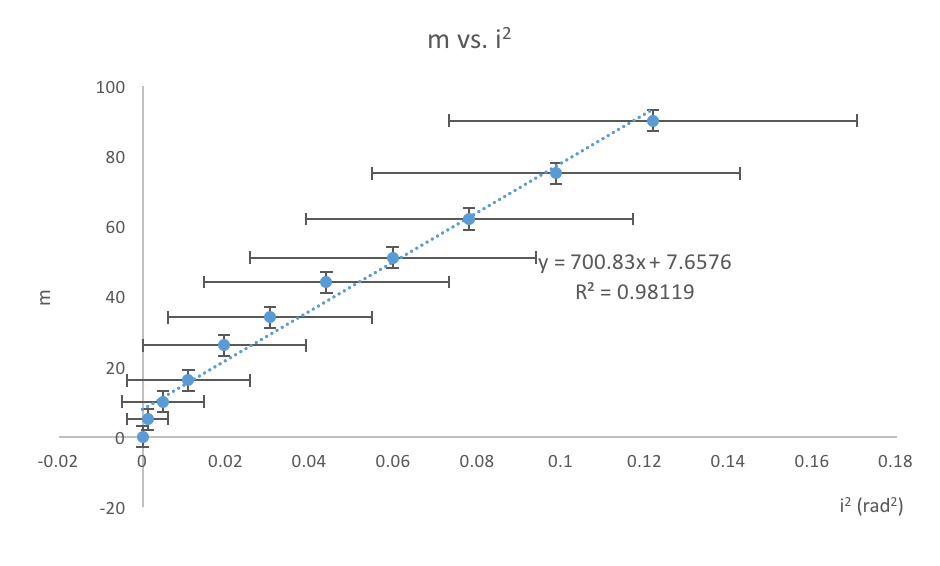
\includegraphics[width=13cm]{Picture5}
		\caption{The number of collapsing fringes with square of the angle of incidence.}
	\end{center}
\end{figure}

Using LINEST function in Excel, we calculated the slope to be $701\pm32$ and y-intercept $8\pm2$. The value for y-intercept to be non-zero was consistent with our small number approximation in our theory. 

For we also used small angle approximation to get the linear relationship between the number of fringes $m$ and the square of incidence angle $i^{2}$, we also needed to consider which part of our data to be used for calculation of refractive index. So we made residual plots as shown in Fig. 6. 
\begin{figure}[!hbt]
	\begin{center}
		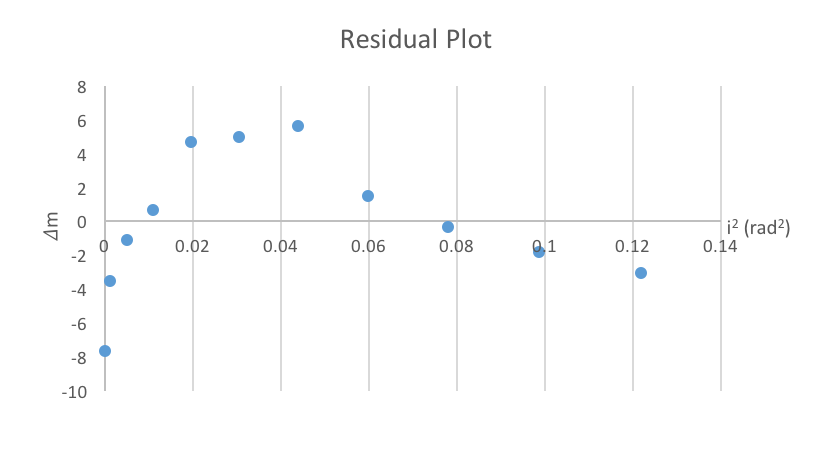
\includegraphics[width=13cm]{Picture6}
		\caption{Residual plot}
	\end{center}
\end{figure}

The clear pattern shown in the residual plot indicated that the relation in fact is not linear, but for simplicity we could get a good approximation with a linear relation when the angle is small. The residual plot gave us a good evaluation of the fitness for the linear relation, with a turning point at around the 7th data point (with $i=0.21$) before which the residuals were increasing and after which decreasing. 

Thus, we only used data with incidence angle smaller than 0.21 rad. The result is shown in Fig. 7. 
\begin{figure}[!ht]
	\begin{center}
		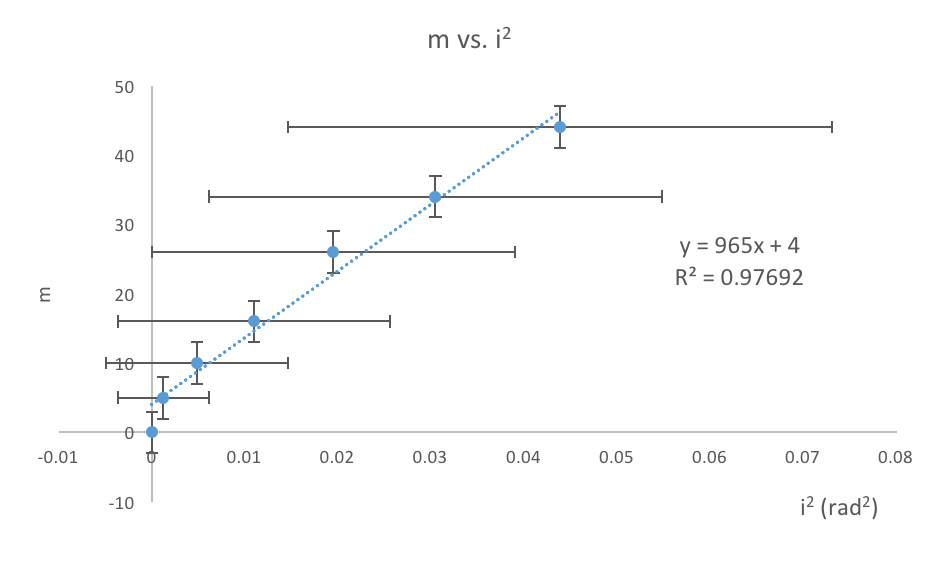
\includegraphics[width=13cm]{Picture7}
		\caption{Refined data plot with incidence angle smaller than $0.21$ rad.}
	\end{center}
\end{figure}

Again using LINEST function in Excel, we got the slope $k=965\pm66$ and y-intercept $b=4\pm1$. For the same reason the non-zero intercept was the result of our approximation in theory. 

Based on Equ. (8) we calculated the refractive index of the acrylic sheet 
\begin{equation}
n=\dfrac{t}{t-k\lambda}=1.43.
\nonumber
\end{equation}

The uncertainty was propagated in quadrature method
\begin{equation}
\sigma_{n}=\sqrt{(\dfrac{\delta{n}}{\delta{k}}\sigma_{k})^{2}+(\dfrac{\delta{n}}{\delta{t}}\sigma_{t})^{2}}=\sqrt{(\dfrac{k\lambda}{(t-k\lambda)^{2}}\sigma_{k})^{2}+(\dfrac{t\lambda}{(t-k\lambda)^{2}}\sigma_{t})^{2}}=0.04.
\nonumber
\end{equation}

So our measured value for the refraction index of the acrylic sheet $n=1.43\pm0.04$ with a relative uncertainty of $3.0\%$. While the expected value was 1.49, our result had a $\left|\dfrac{1.43-1.49}{1.49}\right|=4.2\%$ relative error from the theoretical value. 
%----------------------------------------------------------------------------------------
%	SECTION 5
%----------------------------------------------------------------------------------------
\section{Discussion}
In this lab, we determined the refractive index of air and an acrylic sheet with a Michelson interferometer, a vacuum chamber, and a rotation stage on which we mounted a acrylic sheet. 

\subsection{Experiment a: measure the refraction index of air }
Our determined value for the index of refraction of air was $1.0003\pm0.0104$. It agreed with the expected value of 1.00029 with a relative error of  $0.003\%$.

We concluded our major uncertainty came from the uncertainty of counting the fringes. Since every time after we squeezed the handle, the handle bounced back, causing the pressure to fluctuate violently a small amount of time. It was hard for us to capture the resulted change in the interference pattern in such small time interval, thus, the chance of miscounting increased. 

Since we assumed there was no uncertainty associated with the given value of $L$ (the length of the vacuum chamber), the uncertainty for the refractive index of air was based solely on the calculated slope of the plotting of $m$ as a function of $\Delta{p}$, of which the uncertainty largely consisted of random uncertainties caused by the resolution of the gauge and other random factors. For example, the uncertainty of $\SI{2 }{kPa} $ from the instrument resolution rendered concievably greater relative uncertainty to smaller measure of pressure. These random uncertainties can be reduced by improving the precision or accuracy of the device and averaging a larger amount of observations. 

On the other hand,  there did exist uncertainty regarding the length of the vacuum chamber due to the uneven quality of industrial production, which we did not take into account because its contribution to the total uncertainty was relatively small compared with the random uncertainty induced during experiments. 

So although our measurement agreed with the theoretical value, to improve the precision of our measurement we could either use instruments with greater precision or increase our number of observations. 

\subsection{Experiment b: measure the refraction index of acrylic sheet }
The refractive index of acrylic sheet we determined was $1.43\pm0.04$ with a relative uncertainty of $3.0\%$. Our measurement did not agree with the expected value (1.49) of refractive index of acrylic glass with a relative error of $4.2\%$. 

We attributed our major uncertainty to the systematic uncertainty, which came from the linear model we derived using Taylor and small angle approximation, and on which we based our data analysis. An obvious pattern could be identified in the residual plot of our data, with a clear turning point where the residuals changed from increasing to decreasing. This pattern was a good indication of a non-linear relation between $m$ and $i^{2}$ and demonstrated the systematic error involved in our linear model. Approximation under certain circumstances can yield good results, but often it is hard to judge the bottom line, and that's why it failed in our case. Some characteristics of systematic uncertainties were also shown in our residual plot, with reproducibility and consistency in the same direction. The only way to decrease this kind of error is to apply correction to our function model, which in our case might involve more complicated calculations. 

The poor quality of the instrument also contributed to our uncertainty of measurement. First, the rotation stage was not well secured on the interferometer and could be easily moved when we attampted to rotate the acrylic sheet above. This would result in unexpected change in the angle of incidence without being recorded by the gauge on the rotation stage, increasing the uncertainty within the incidence angle. Moreover, it was hard to make controlled and smooth rotation of the sheet manually. The fringes would flash by under a sudden change of angle without being noticed and resulted in a greater chance of miscounting. The interference pattern also passed by at a greater rate as the angle displacement became larger (which was evidenced in the formula with the number of fringes $m$ proportional to the square of incidence angle $i$). So as the angle became larger, there would be more fringes passing by for the same angle displacement. The chance of miscounting also increased with a greater amount of fringes to be count. We can improve our experiment with more accurate and refined instrument, like using a vernier scale for the angle measurement and auto-rotation stage that automatically rotates at a set rate. 

\end{document}